%!TEX root = main.tex
\chapter{Results}
\label{chap:results}
In this chapter we will show and discuss the results of the work we have done in this thesis.

We will start by looking at the train and test sets of the four dataset (see \autoref{tab:model_delimitation} and below) and describe what we did about class imbalance. Then we describe and interpret our results and we end the chapter with a brief summary of our findings. 

From \autoref{chap:methods} we have found the following datasets and model pairs based on the available data (see also \autoref{tab:model_overview} and \autoref{tab:model_delimitation}):
\begin{enumerate}
\item Test data
\begin{enumerate}
\item without user-filtering \\\textbf{Model pair: TP-1}
\item with user-filtering using cross-occupancy of 40\% \\\textbf{Model pair: TP-2}
\end{enumerate}
\item Production data
\begin{enumerate}
\item without user-filtering \\\textbf{Model pair: PP-1}
\item with user-filtering using cross-occupancy of 10\% \\\textbf{Model pair: PP-1}
\end{enumerate}
\end{enumerate}


For our test data without user-filtering we found a training set with 1798 negative samples (did not meet) and 9203 positive samples (did meet). In our test set we found a more moderate 5513 negative samples (did not meet) and 1674 positive samples (did meet).

Using test data with user-filtering in just September we found a training set with 118 that did not meet and 95 that did meet. The test set consisted of 151 that did not meet and 98 that did meet. 

Using production data without user-filtering we found 5585 that did not meet and 10907 that did meet for our training set, for our test set we found 9148 that did not meet and 10028 that did meet.

Using production data with user-filtering we found 403 that did not meet and 4533 that did meet for our train set and 402 that did not meet and 4630 that did meet for our test set.

The datasets composed from the test data have more negative samples than positive samples. In TP-1 the difference is more pronounced than in TP-2, except of the training set. In the production data, we have the opposite. Here we have more positive samples than negative. \\
This shows we have a class impalance problem since the dataset are imbalanced. Due to this, the Logistic Regression classifier we trained initially predicted the largest prevalent class, in our training dataset. The next section explains this problem and how we dealt with it. 


\section{Class Imbalance Problem}
\label{sec:class_imbalance_problem}
The Class Imbalance Problem is when the total number of samples for one class greatly exceeds the number of samples for a different class. A number of techniques can be used to handle the class imbalance problem, two of the most common techniques are called oversampling and undersampling\cite{tan2006introduction}. In oversampling you sample the minor sample with replacement until there is an equal number of positive and negative samples. In undersampling you randomly sample from the major class $N$ times where $N$ is the number of minor classes. We will try to use undersampling when training our models.

\section{Performance metrics}
\label{sec:performance_metrics}
We utilize the precision and recall metrics for evaluating the performance of our models as well as AUC of the ROC Curve.

\subsection{Receiver Operating Characteristic (ROC)}
The Receiver Operating Characteristic or ROC in short, illustrates the performance of a binary classifier in terms of the true positive rate (TPR, also called recall) plotted against the false positive rate (FPR) at different discrimination thresholds. As points on the ROC-curve represents different thresholds with an associated (TPR,FPR) pair it allows us to see different trade-offs between TPR and FPR. The ROC curve is useful for comparing the relative performance of different classifiers\cite{tan2006introduction} The area under the curve (AUC) represents the probability that a classifier will rank a random positive sample higher than a negative sample, assuming positive ranks higher. An AUC of 0.5 would mean the model would just randomly guess the class of each sample. We will use the ROC AUC as a metric for comparing our different models.

\subsection{Precision and Recall}
Precision or the positive predictive value (PPV) is a metric that measures the number of a given class that are correctly identified in proportion to the number of classes that are predicted to be that class.

Recall, or the true positive rate (TPR), is a metric that measures the number of a given class that are correctly identified as that class. PPV and TPR is defined in \autoref{eq:precision} and \autoref{eq:recall} respectively. 

\begin{equation}
\label{eq:precision}
PPV=\frac{TP}{TP+FP}
\end{equation}

\begin{equation}
\label{eq:recall}
TPR=\frac{TP}{TP+FN}
\end{equation}

$TP$ is true positive. It is the number of records predicted as 'did meet', which really is 'did meet'. $FP$ is the false positive which is the number of records predicted to be 'did meet' which actually is 'did not meet'. Last we have $FN$ that is the false negative. Here it is the number of records predicted to be 'did not meet' which actually is from 'did meet'. 

Thus precision show how good the classifier is to predict 'did meet' of those is has classified as 'did meet' i.e. fraction of records that actually is the 'did meet' in the group the classifier has classified as 'did meet'. Recall show how good the result are by looking at how complete the results are i.e. the fraction of correct predicted 'did meet' over all predicted records (both records which is realy 'did meet' and those which is 'did not meet') of the 'did meet' class. \\

We aim for high precision and high recall as it means low number of false positive errors and few positively misclassified as negative class\cite{tan2006introduction}. 

As a summary we have the $F_1$ score which is the harmonic mean of the precision an recall. Since the score tence to be closer to the lowest value (of precision and recall), a high $F_1$ score ensures precision and recall to be reasonably high\cite{tan2006introduction}. 
The $F_1$ score is defined as follows

\begin{equation}
\label{eq:f1_score}
F_1=\frac{2*TP}{2*TP+FP+FN}
\end{equation}
$FP$ is the number of records 'did not meet' wrongly predicted as 'did meet'. 

In Table \ref{table:models_performance_report} and \ref{table:models_performance_report_undersampling} we can see the performance metrics of the different classifiers for the positive (did meet) and negative class (did not meet), in the dataset without undersampling and the dataset with undersampling respectively.

\begin{table}[H]
\centering
\begin{tabular}{|c|c|c|c|c|c|c|c|}
\hline
\textbf{Model} & \textbf{PPV} & \textbf{TPR} & \textbf{$F_1$-score}   \\
\specialrule{.20em}{.0em}{.0em}
LR in TP-1    & 0.25 & 0.67 & 0.37 \\
\hline
RF in TP-1    & 0.47 & 0.15 & 0.23 \\
\specialrule{.15em}{.0em}{.0em} 
LR in TP-2    & 0.53 & 0.68 & 0.59 \\
\hline
RF in TP-2    & 0.54 & 0.52 & 0.53 \\
\specialrule{.15em}{.0em}{.0em}
LR in PP-1    & 0.66 & 0.74 & 0.70 \\
\hline
RF in PP-1    & 0.65 & 0.61 & 0.63 \\
\specialrule{.15em}{.0em}{.0em}
LR in PP-2    & 0.94 & 0.81 & 0.87 \\
\hline
RF in PP-2    & 0.93 & 0.99 & 0.96 \\
\hline
\end{tabular}
\caption{Models performance metrics without undersampling}
\label{table:models_performance_report}
\end{table}
We can see the Random Forest (RF) has higher precision than the Logistic Regression (baseline) in almost all the pairs (except in PP-2. We come back to this later). 
The recall is higher for the baseline in all except in PP-2.

In TP-1 the RF is the worst of the RF's, when we compare it with the other RF's. It has better precision than the baseline (which has quite bad precision). This means, it has lower number of 'did meets' which in fact was 'did not meet' than the baseline, which is good. On the other hand, it has way worse recall than the baseline meaning, that is has more 'did meets' which been misclassified as 'did not meets'. 

In TP-2 the recall of the RF is way better, but still worse than baseline. Precision is also a little better and infact a little better than the baseline. 

In PP-1 and PP-2 we can see these have better performance than the other two in both baseline and Random Forest. As mentioned earlier, the precision for the RF in PP-2 are slight worse than the baseline. The racall is way better and the $F_1$ score shows a better performance than the baseline. 

The $F_1$ score shows that the baseline is better in all the pairs except for PP-2. 

\begin{table}[H]
\centering
\begin{tabular}{|c|c|c|c|c|c|c|c|}
\hline
\textbf{Model} & \textbf{PPV +} & \textbf{TPR +} & \textbf{f-score}    \\
\specialrule{.20em}{.0em}{.0em}
LR in TP-1    & 0.25 & 0.67 & 0.37 \\
\hline
RF in TP-1    & 0.28 & 0.53 & 0.37 \\
\specialrule{.15em}{.0em}{.0em} 
LR in TP-2    & 0.53 & 0.68 & 0.59 \\
\hline
RF in TP-2    & 0.53 & 0.62 & 0.57 \\
\specialrule{.15em}{.0em}{.0em}
LR in PP-1    & 0.66 & 0.74 & 0.70 \\
\hline
RF in PP-1    & 0.66 & 0.56 & 0.61 \\
\specialrule{.15em}{.0em}{.0em}
LR in PP-2    & 0.94 & 0.81 & 0.87 \\
\hline
RF in PP-2    & 0.95 & 0.89 & 0.92 \\
\hline
\end{tabular}
\caption{Models performance metrics with undersampling}
\label{table:models_performance_report_undersampling}
\end{table}

\subsection{Feature importance}
The Random Forest model allows for finding the relative importance of the different features. The depth of a feature in the trees can be used to determine importance as features at the top of of the tree contributes to the prediction decision over a larger fraction of samples. The average is then computed from each tree in the forest to obtain the final feature importances.
Figure \ref{fig:feature_importances} shows the mean of the feature importances of the random forest of PP2. We can see the features which contribute most are features 8 (mutual co-occurrences), 14 (specificity), 5 (co-occurrences weighted), 4 (weighted frequency), 7 (number of co-occurrences), 2 (diversity), 3 (unique co-occurrences). Feature 12 (number of evenings) contributes very little and 13 (number of weekends) seems to have no variance.
\begin{figure}[H]
    \hspace*{-1.0cm}
    \centering
    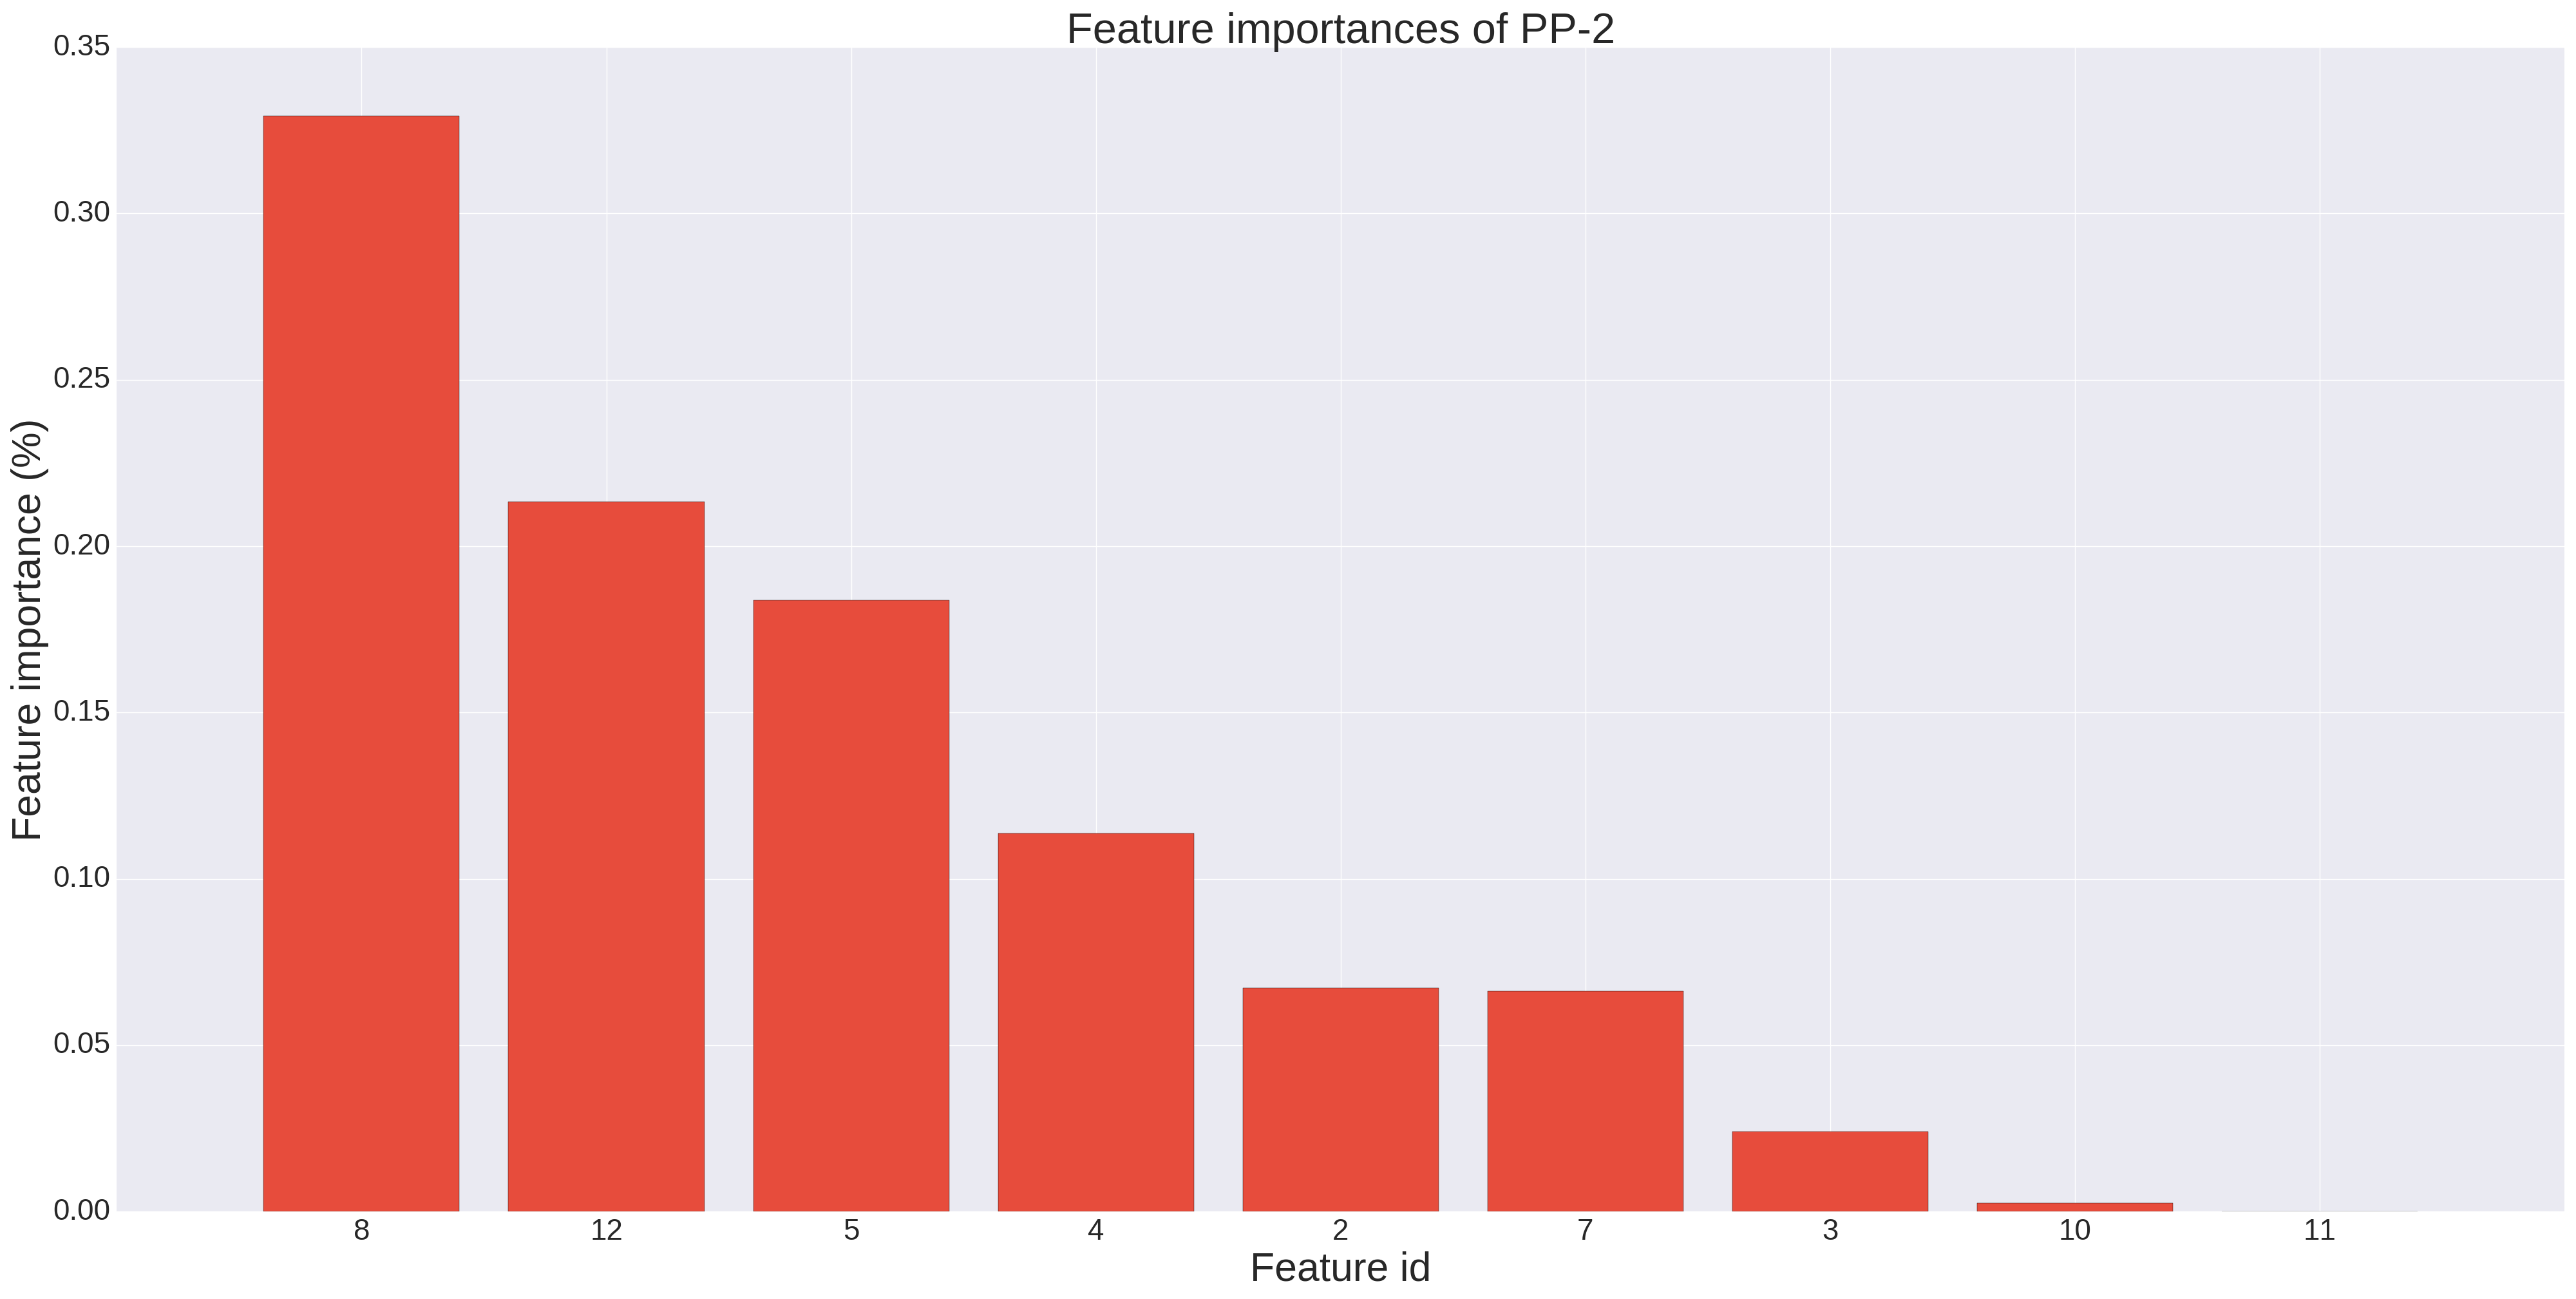
\includegraphics[scale=0.10]{feature_importance_PP2}
    \caption{Feature importances of random forest for PP2}
    \label{fig:feature_importances}
\end{figure}

In the next plots we try to look at the differences in features between the meet and non-meets.
Looking at Figure \ref{fig:feature_boxplots1} to \ref{fig:feature_boxplots4} we can see features which have very little variance like number of weekends, evenings and common travels. Co-occurrences weighted and timely arrival and leaving seems to have similar values, we can note a slightly higher mean for the did not meet class. The homophily features seems very similar as well. Diversity, weighted frequency have very extreme outliers, a large diversity signifies a user pair with a very large number of locations between them. Specificity has extreme outliers as some of the previous features. App usage similarity strangely enough seems to be more similar for the did not meet class, this could be because it does not account for popular apps used by both groups. Number of co-occurrences, mutual co-occurrences and specificity seems to have higher values for the did meet class, and two of the three also contributed most to the importances for our features.

\begin{figure}[H]
    \hspace*{-1.0cm}
    \centering
    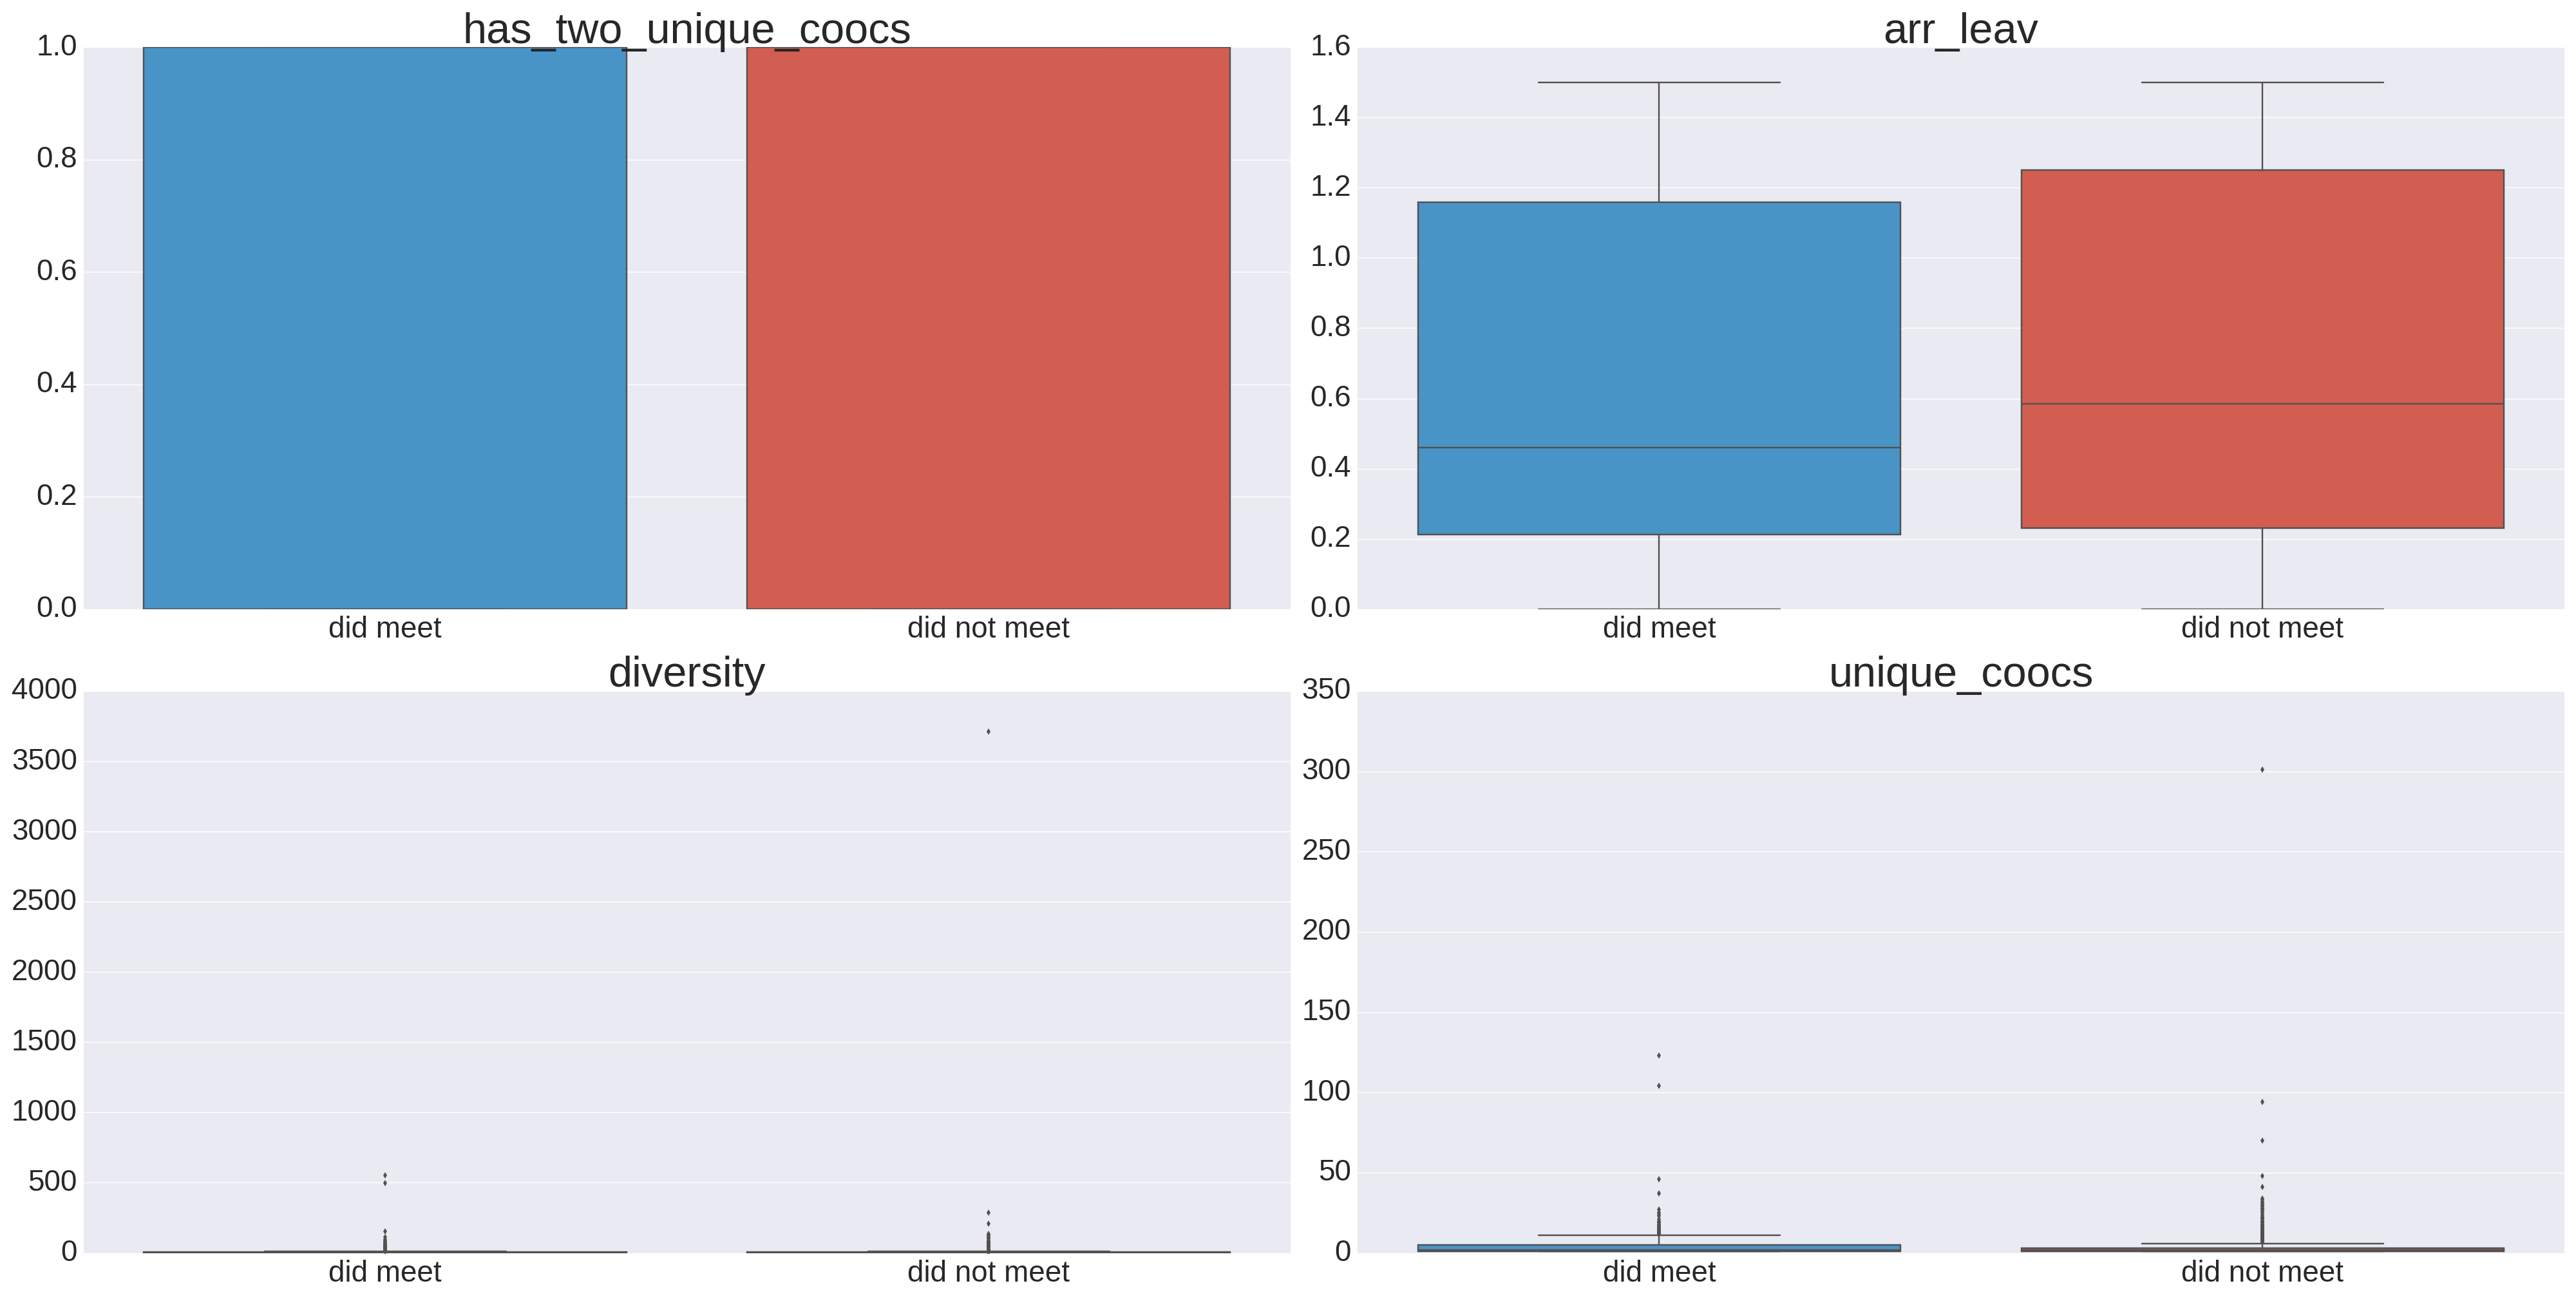
\includegraphics[scale=0.15]{feature_boxplots1}
    \caption{Boxplots of features of TP2}
    \label{fig:feature_boxplots1}
\end{figure}

\begin{figure}[H]
    \hspace*{-1.0cm}
    \centering
    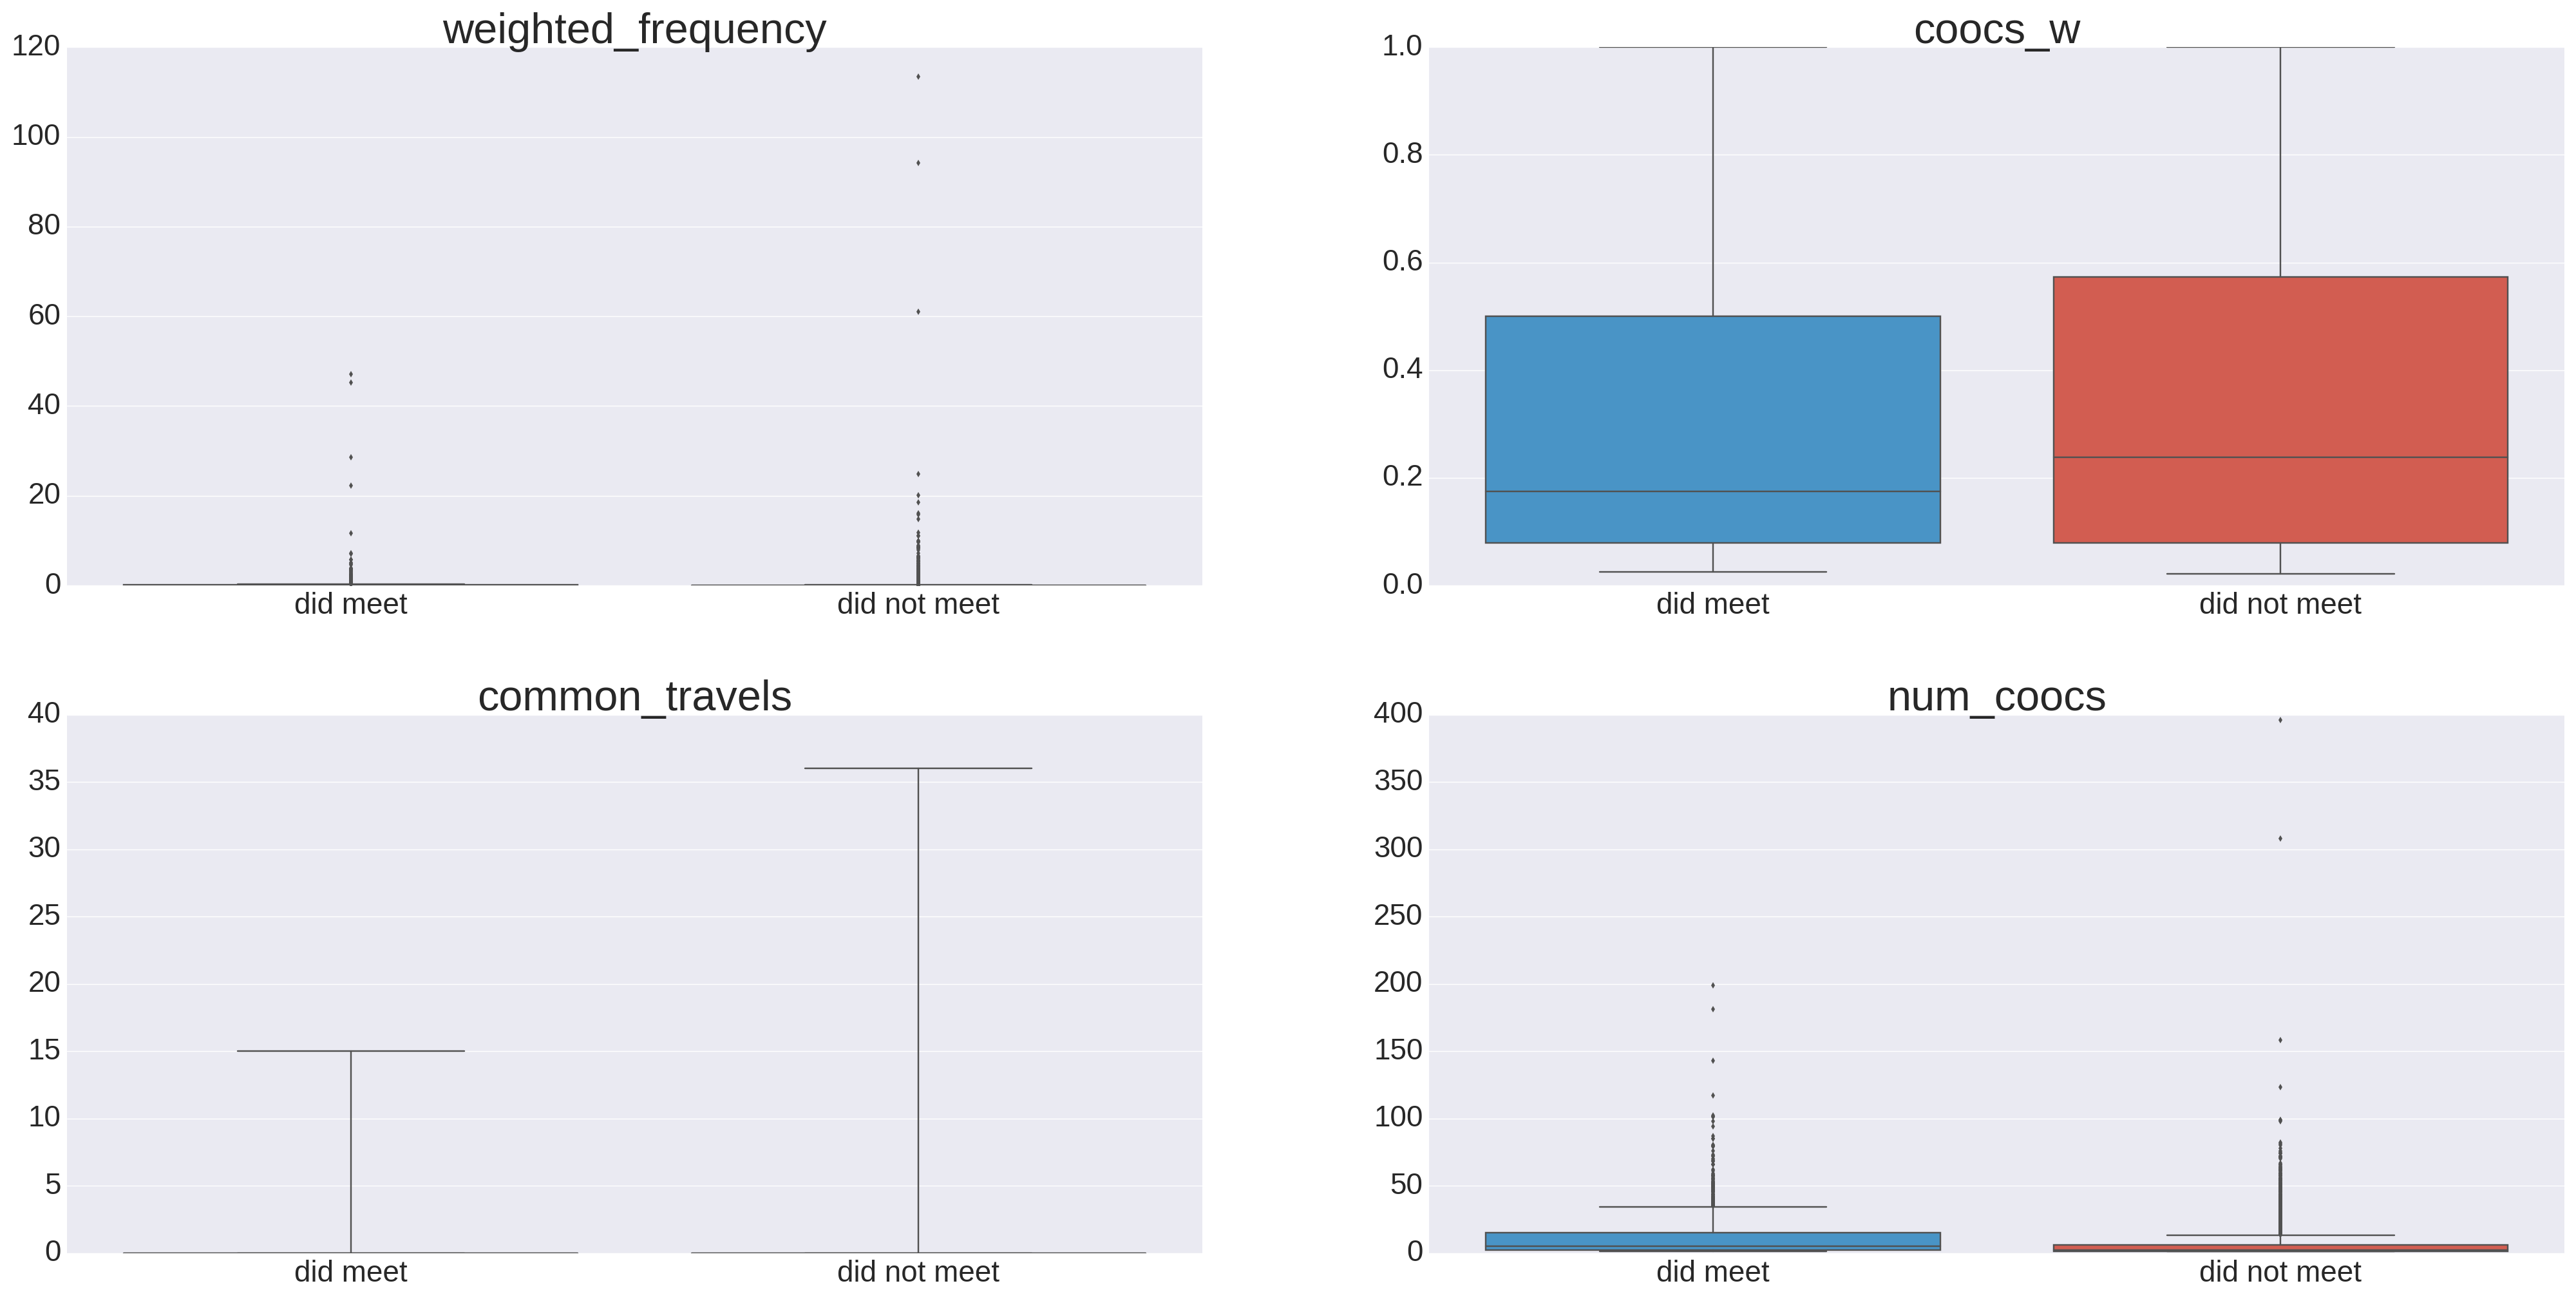
\includegraphics[scale=0.15]{feature_boxplots2}
    \caption{Boxplots of features of TP2}
    \label{fig:feature_boxplots2}
\end{figure}
\begin{figure}[H]
    \hspace*{-1.0cm}
    \centering
    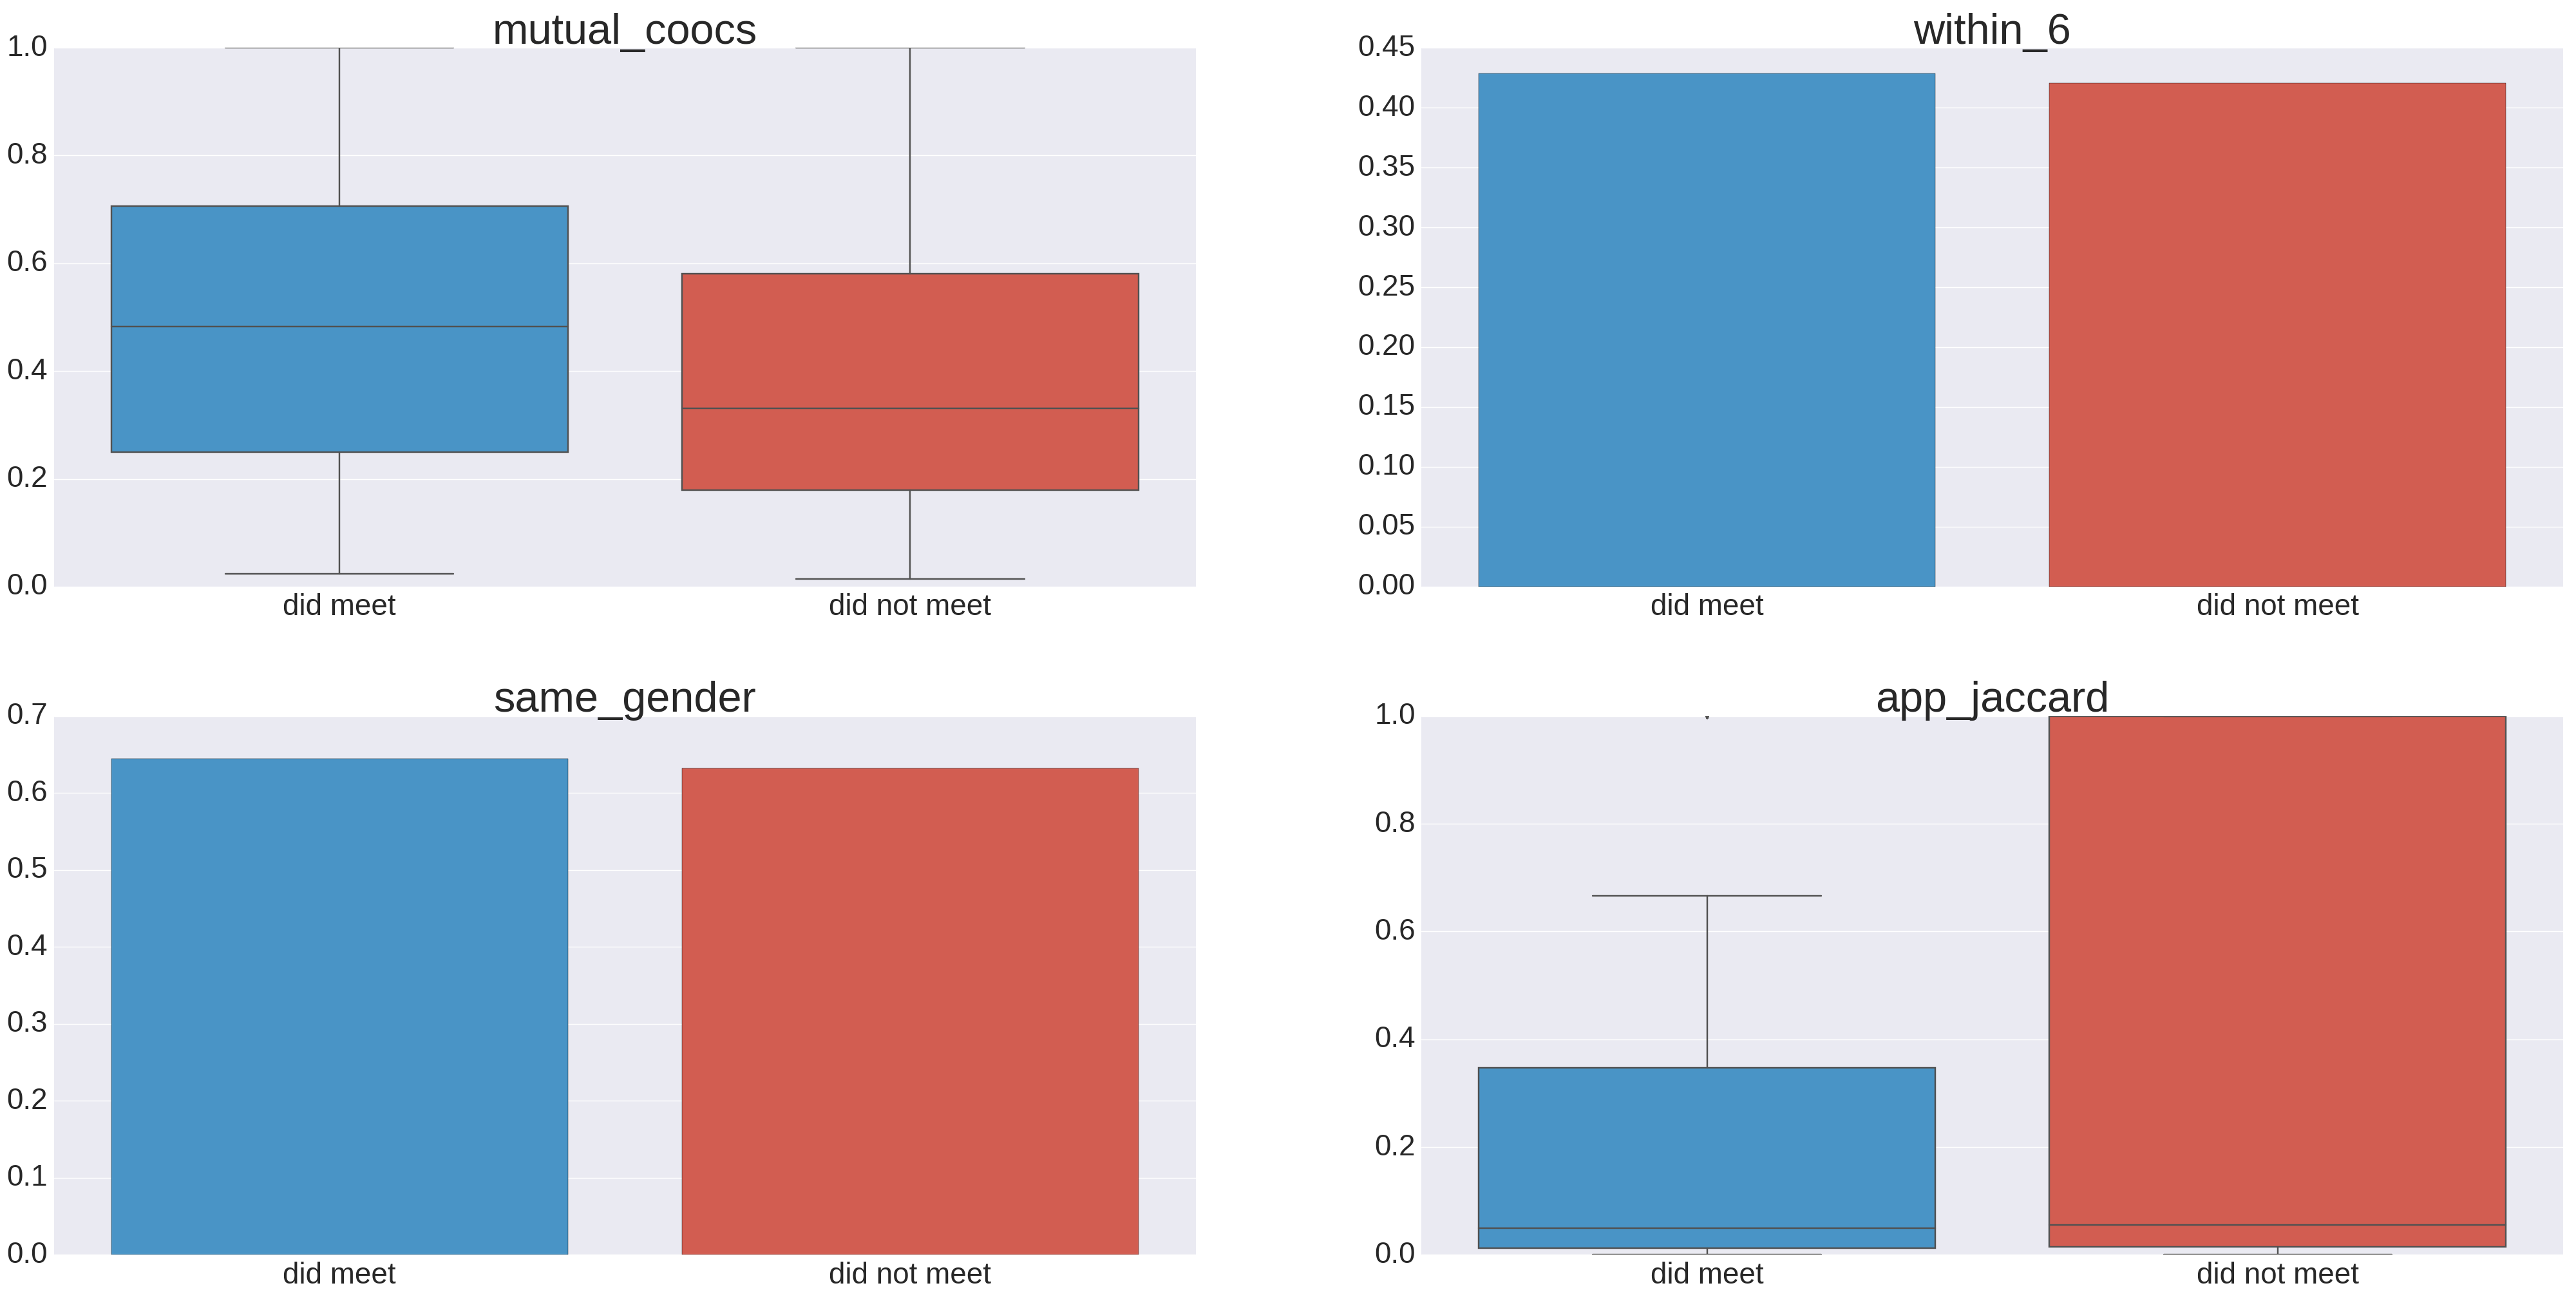
\includegraphics[scale=0.15]{feature_boxplots3}
    \caption{Boxplots of features of TP2}
    \label{fig:feature_boxplots3}
\end{figure}
\begin{figure}[H]
    \hspace*{-1.0cm}
    \centering
    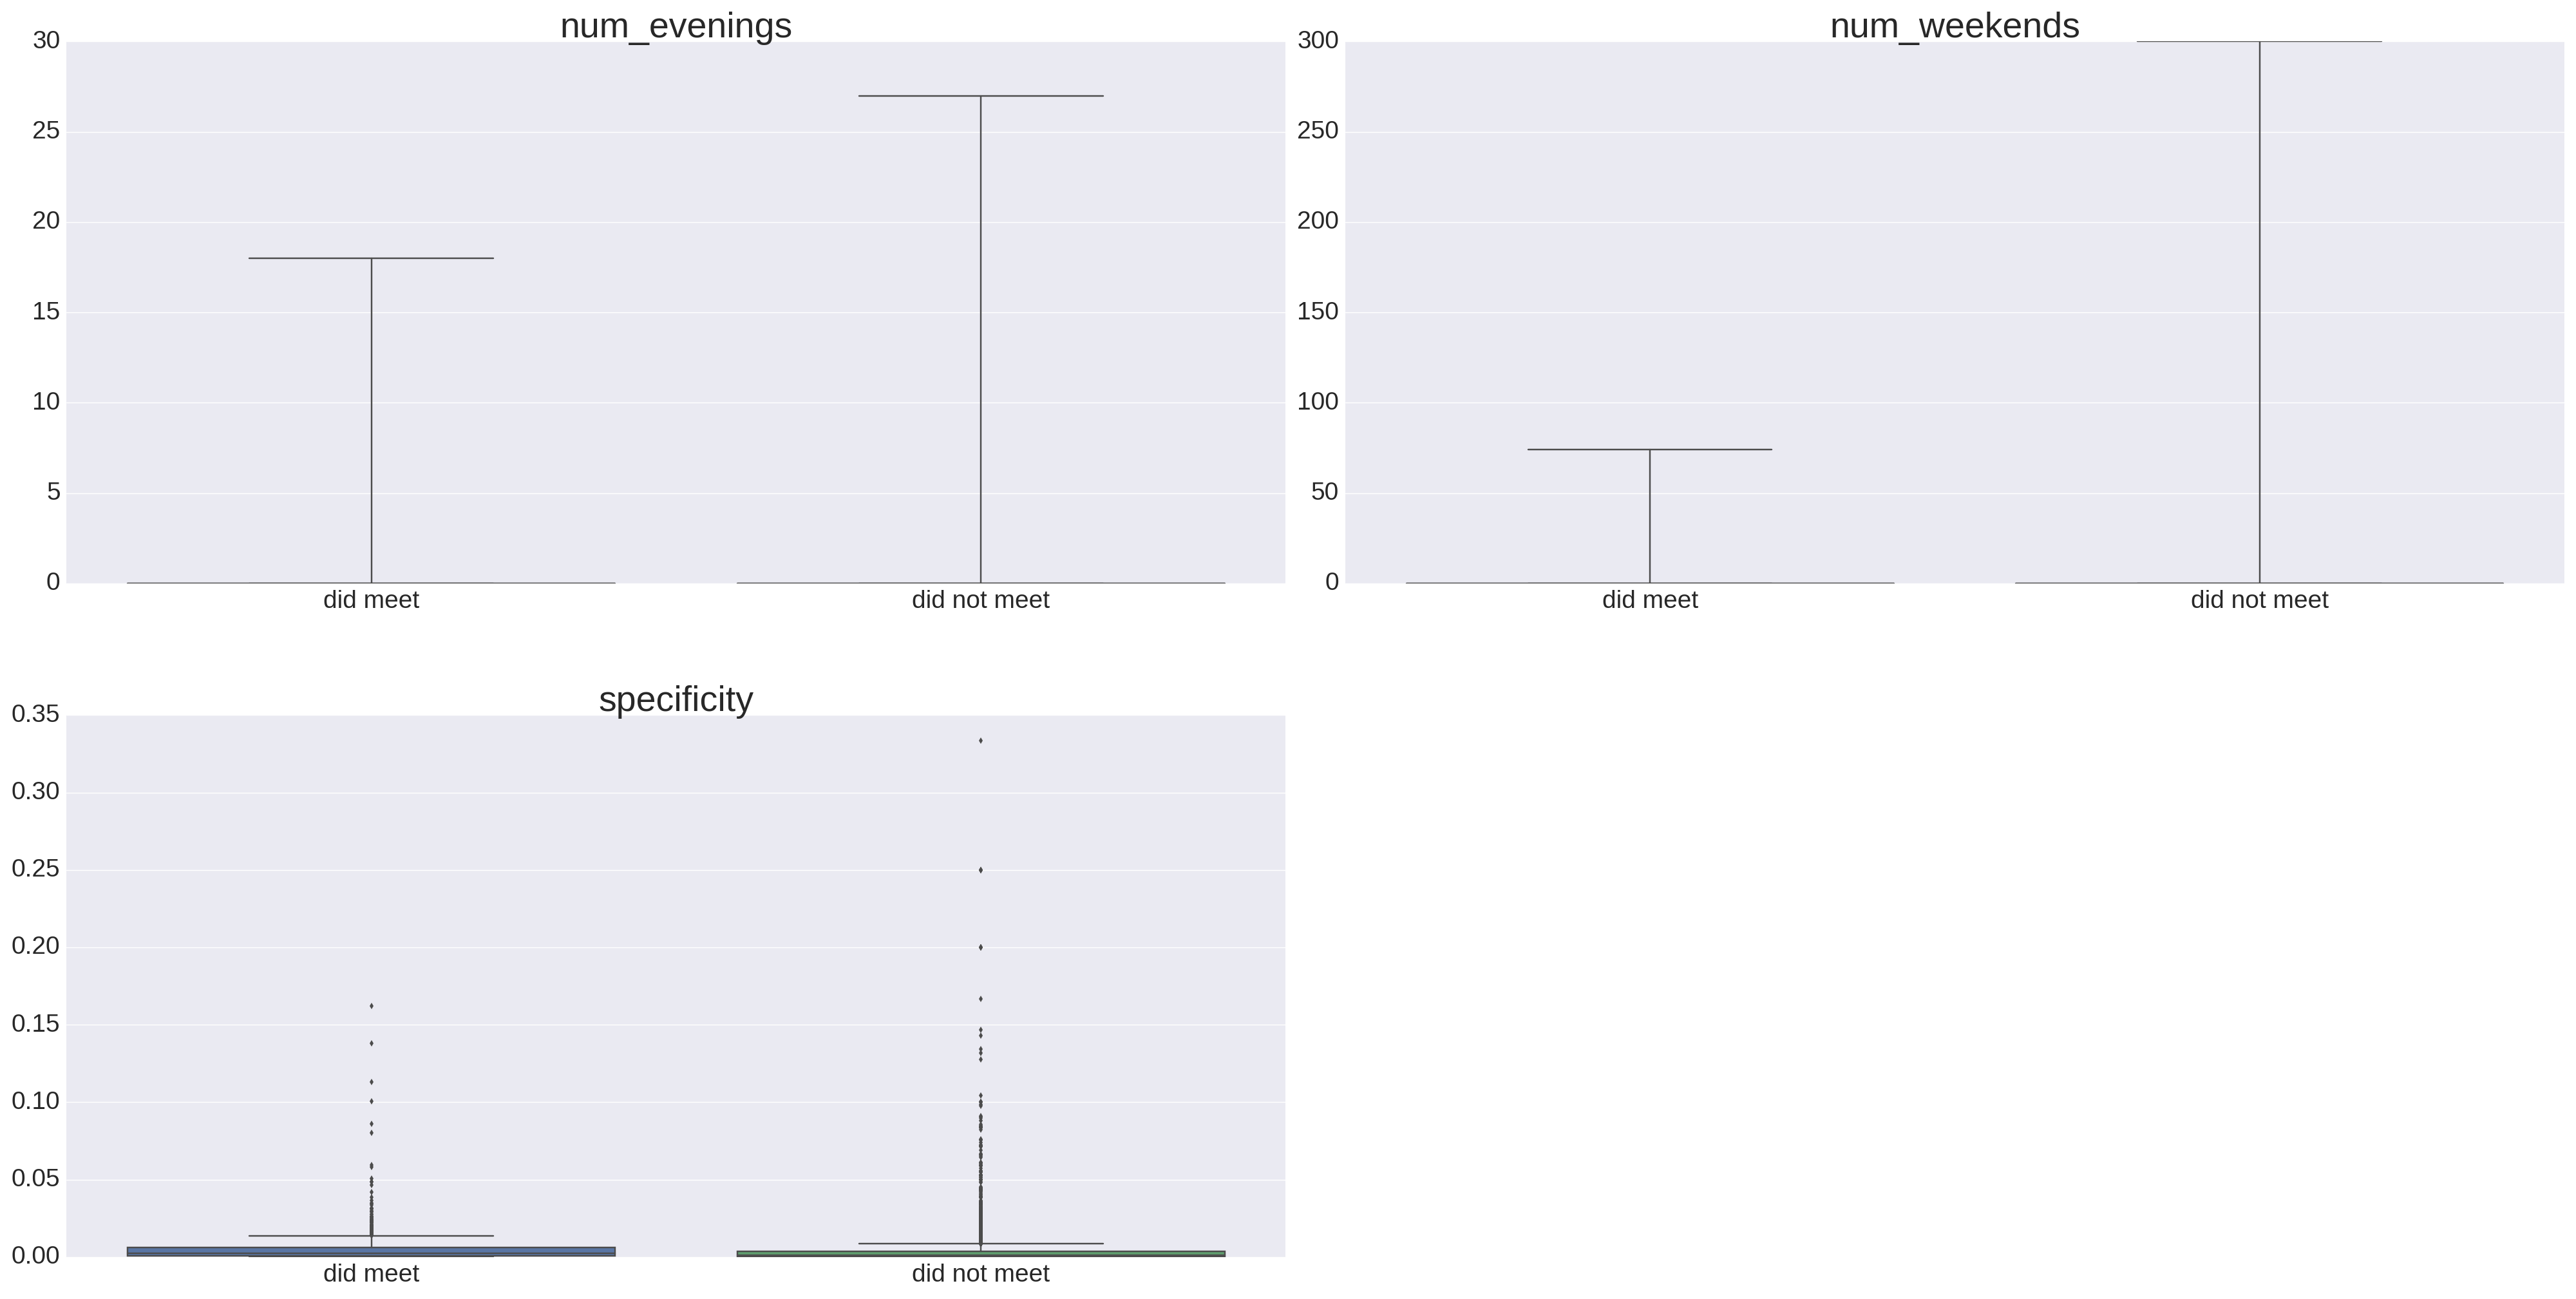
\includegraphics[scale=0.15]{feature_boxplots4}
    \caption{Boxplots of features of TP2}
    \label{fig:feature_boxplots4}
\end{figure}
In Figure \ref{fig:rocs} we have plotted the ROC curve and ROC AUC for the different model pairs, we have also plotted the curve of a randomly guessing classifier for comparison. Figure \ref{fig:rocs_undersampling} shows the same models performance, where the datasets most prevalent class have been undersampled. We used randomized search to find the optimal hyper-parameters in the Random Forest models, choosing from \textit{gini} or\textit{entropy} and $1-9$ max features for each split. The randomized search runs for 20 iterations where each iteration performs a 3-fold cross-validation to validate the parameters of the model, we used ROC AUC as the scoring function. When the best parameters for the model are found, 2-fold cross-validation is performed to validate the model.

\begin{figure}[H]
    \hspace*{-1.0cm}
    \centering
    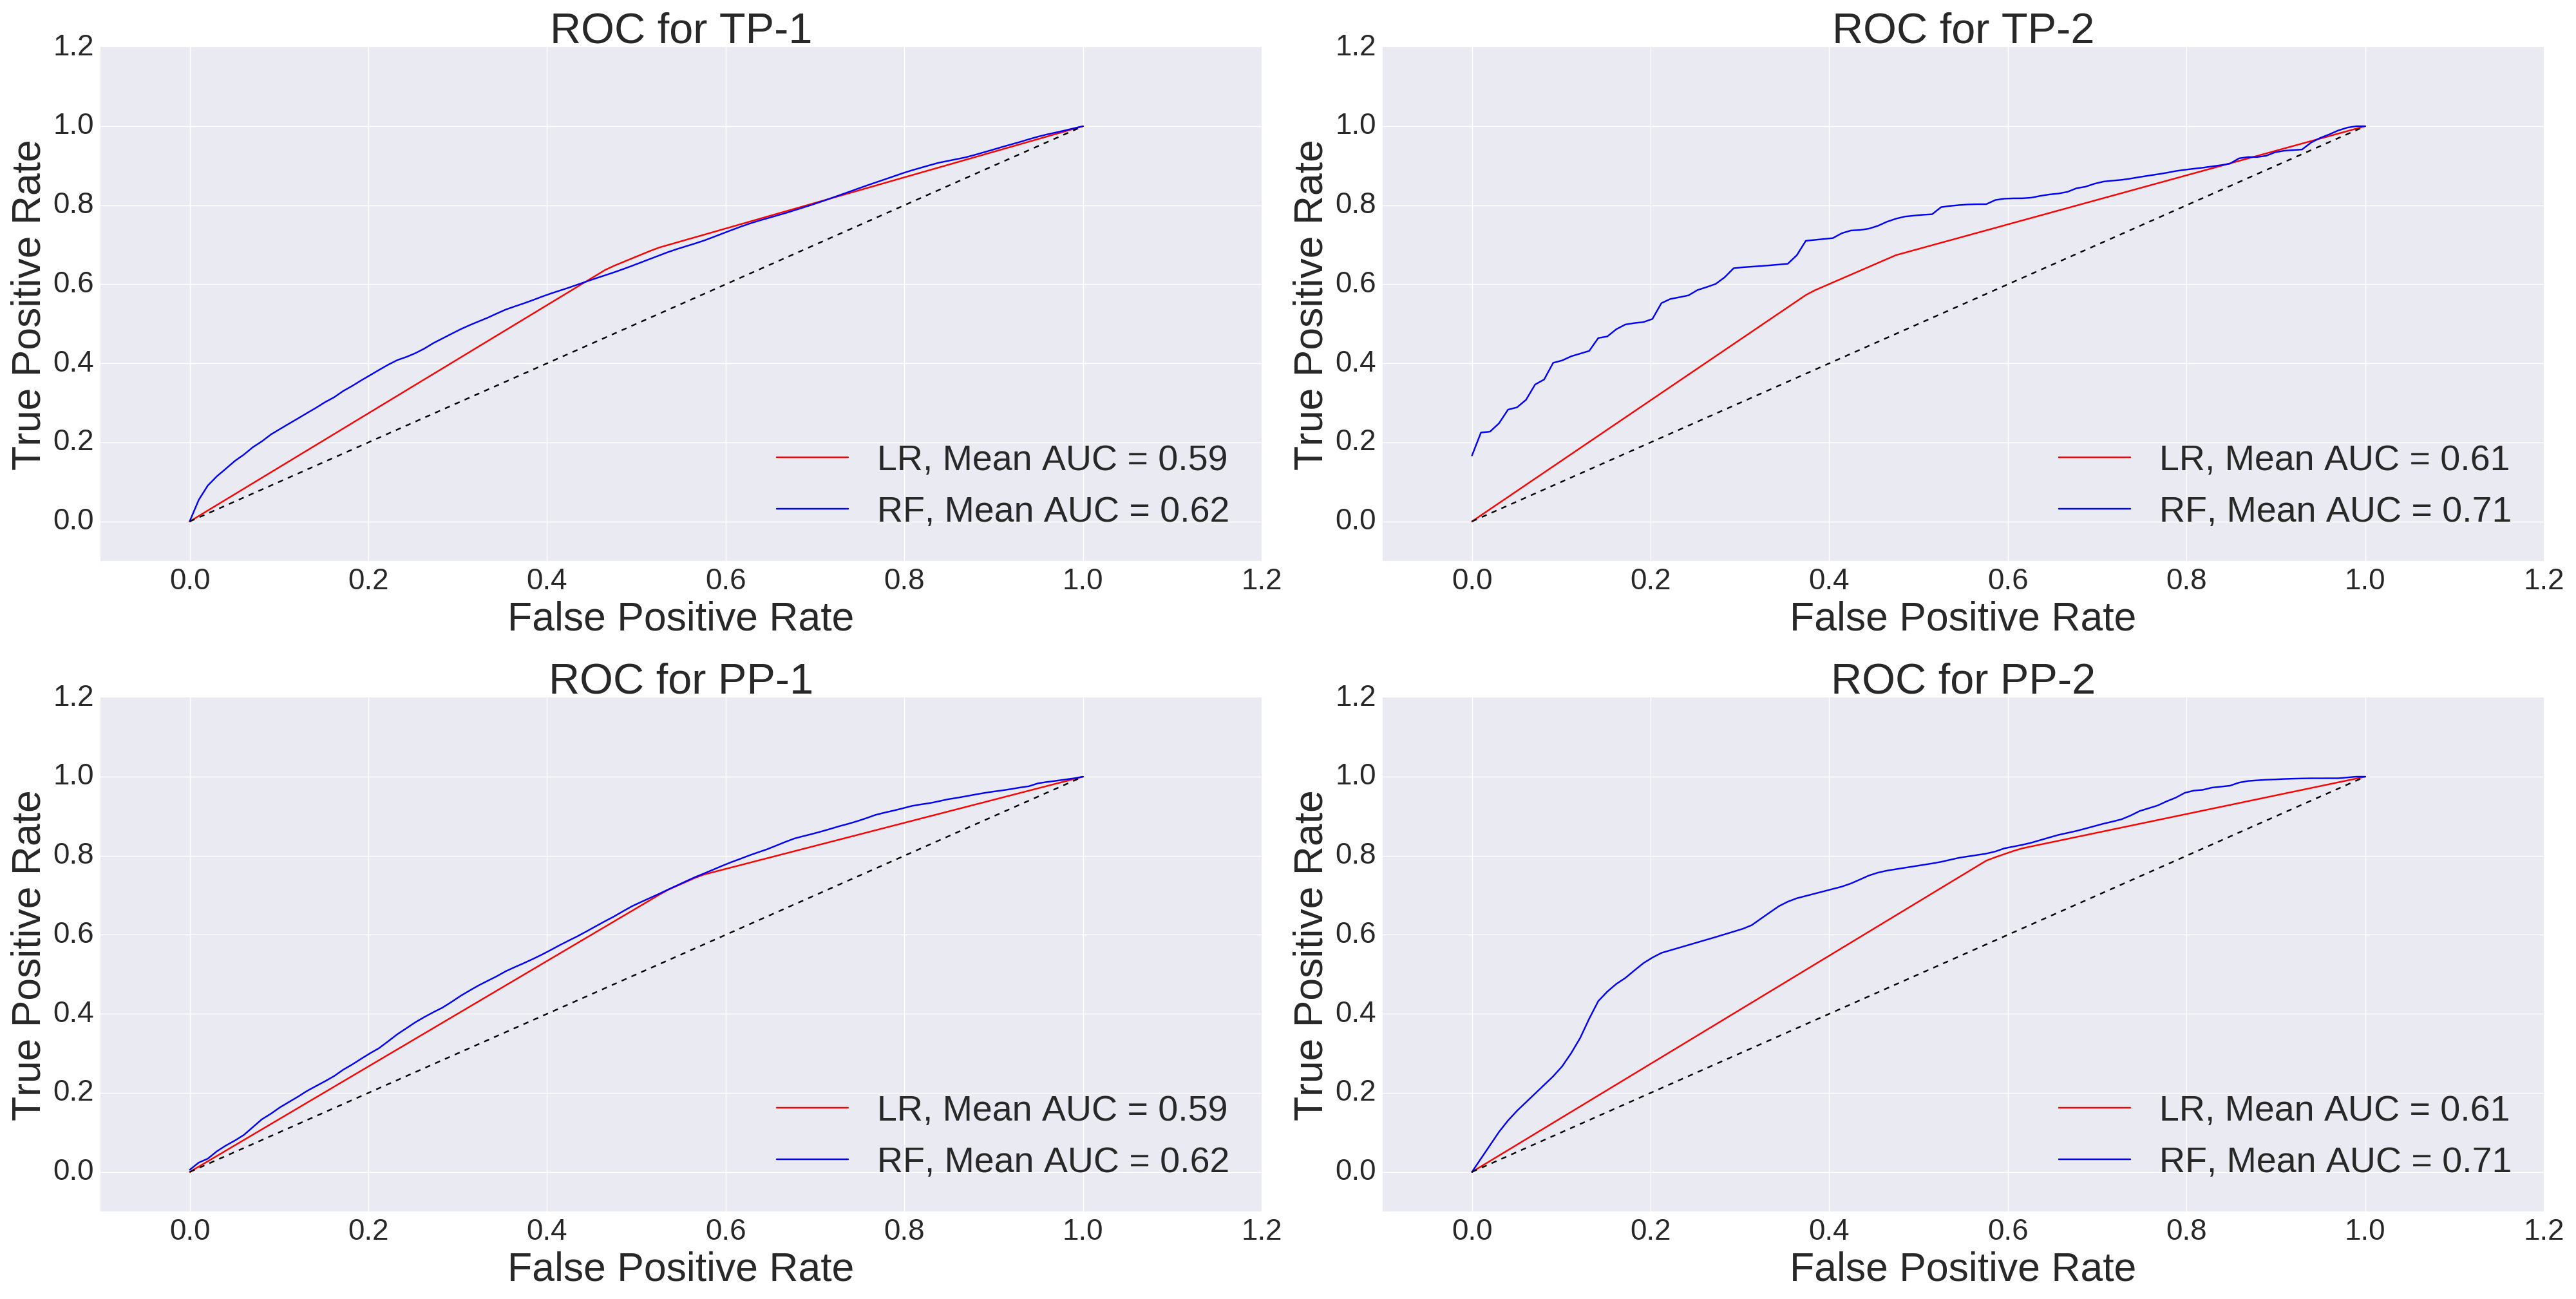
\includegraphics[scale=0.15]{ROCS}
    \caption{mean ROC AUC of Logistic Regression (LR) and Random Forest (RF) in the four model-pairs (TP-1, TP-2, PP-1, PP-2) using randomized search for hyper-parameter optimization (internal loop with 3-fold cross-validation) and 2-fold cross-validation. }
    \label{fig:rocs}
\end{figure}
\begin{figure}[H]
    \hspace*{-1.0cm}
    \centering
    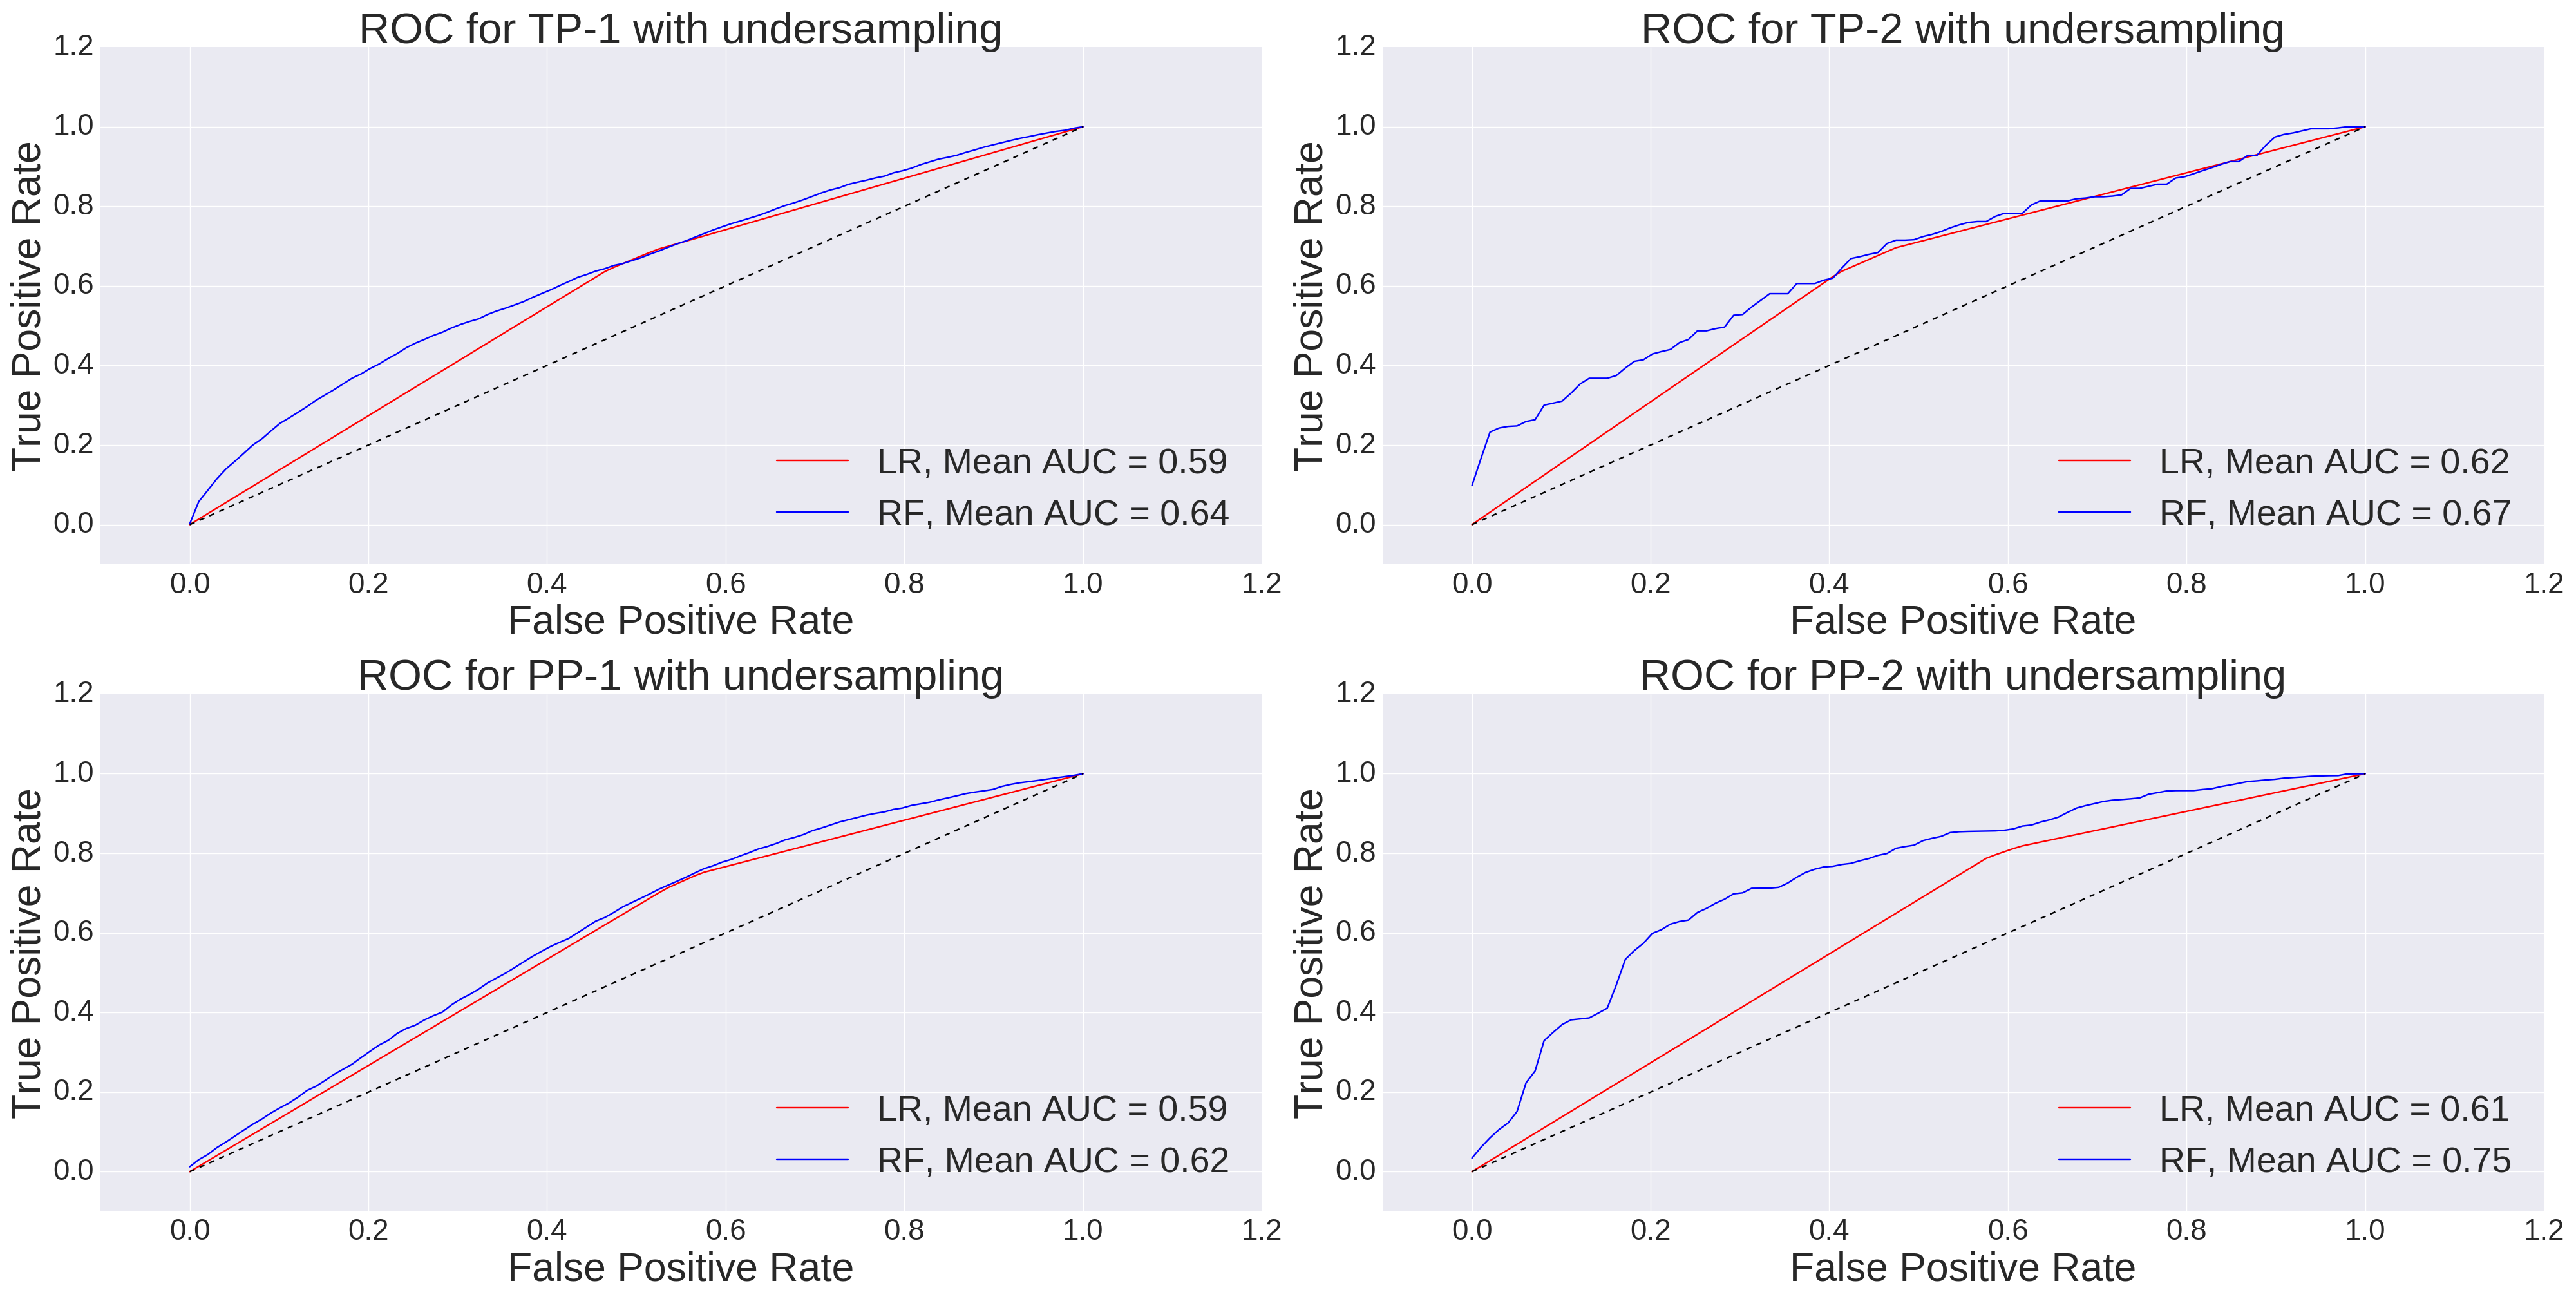
\includegraphics[scale=0.15]{ROCS_undersampling}
    \caption{mean ROC AUC of Logistic Regression (LR) and Random Forest (RF) in the four model-pairs (TP-1, TP-2, PP-1, PP-2) using randomized search for hyper-parameter optimization (internal loop with 3-fold cross-validation) and 2-fold cross-validation, and with undersampling of the most prevalent class}
    \label{fig:rocs_undersampling}
\end{figure}
\section{Summary}